\subsection{Overfitting}

\begin{frame}[c]{}
  \begin{center}
    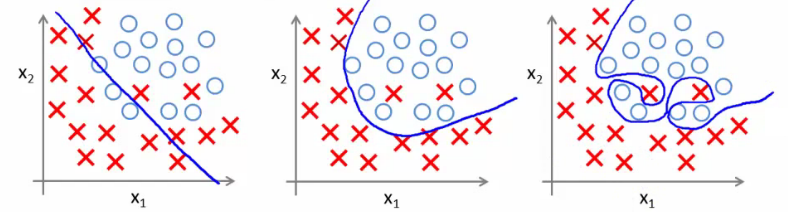
\includegraphics[scale=0.6]{./pictures/overfitting.png}
  \end{center}
\end{frame}

\begin{frame}
  \begin{equation*}
    E(w) = -y \log(o) - (1 - y)(1 - o) \mathbf{+ \lambda \displaystyle\sum_{i, j}{w_{ij}^2}}
  \end{equation*}
\end{frame}

\subsection{Local minima}

\begin{frame}[c]{Local Minima}
  \begin{center}
    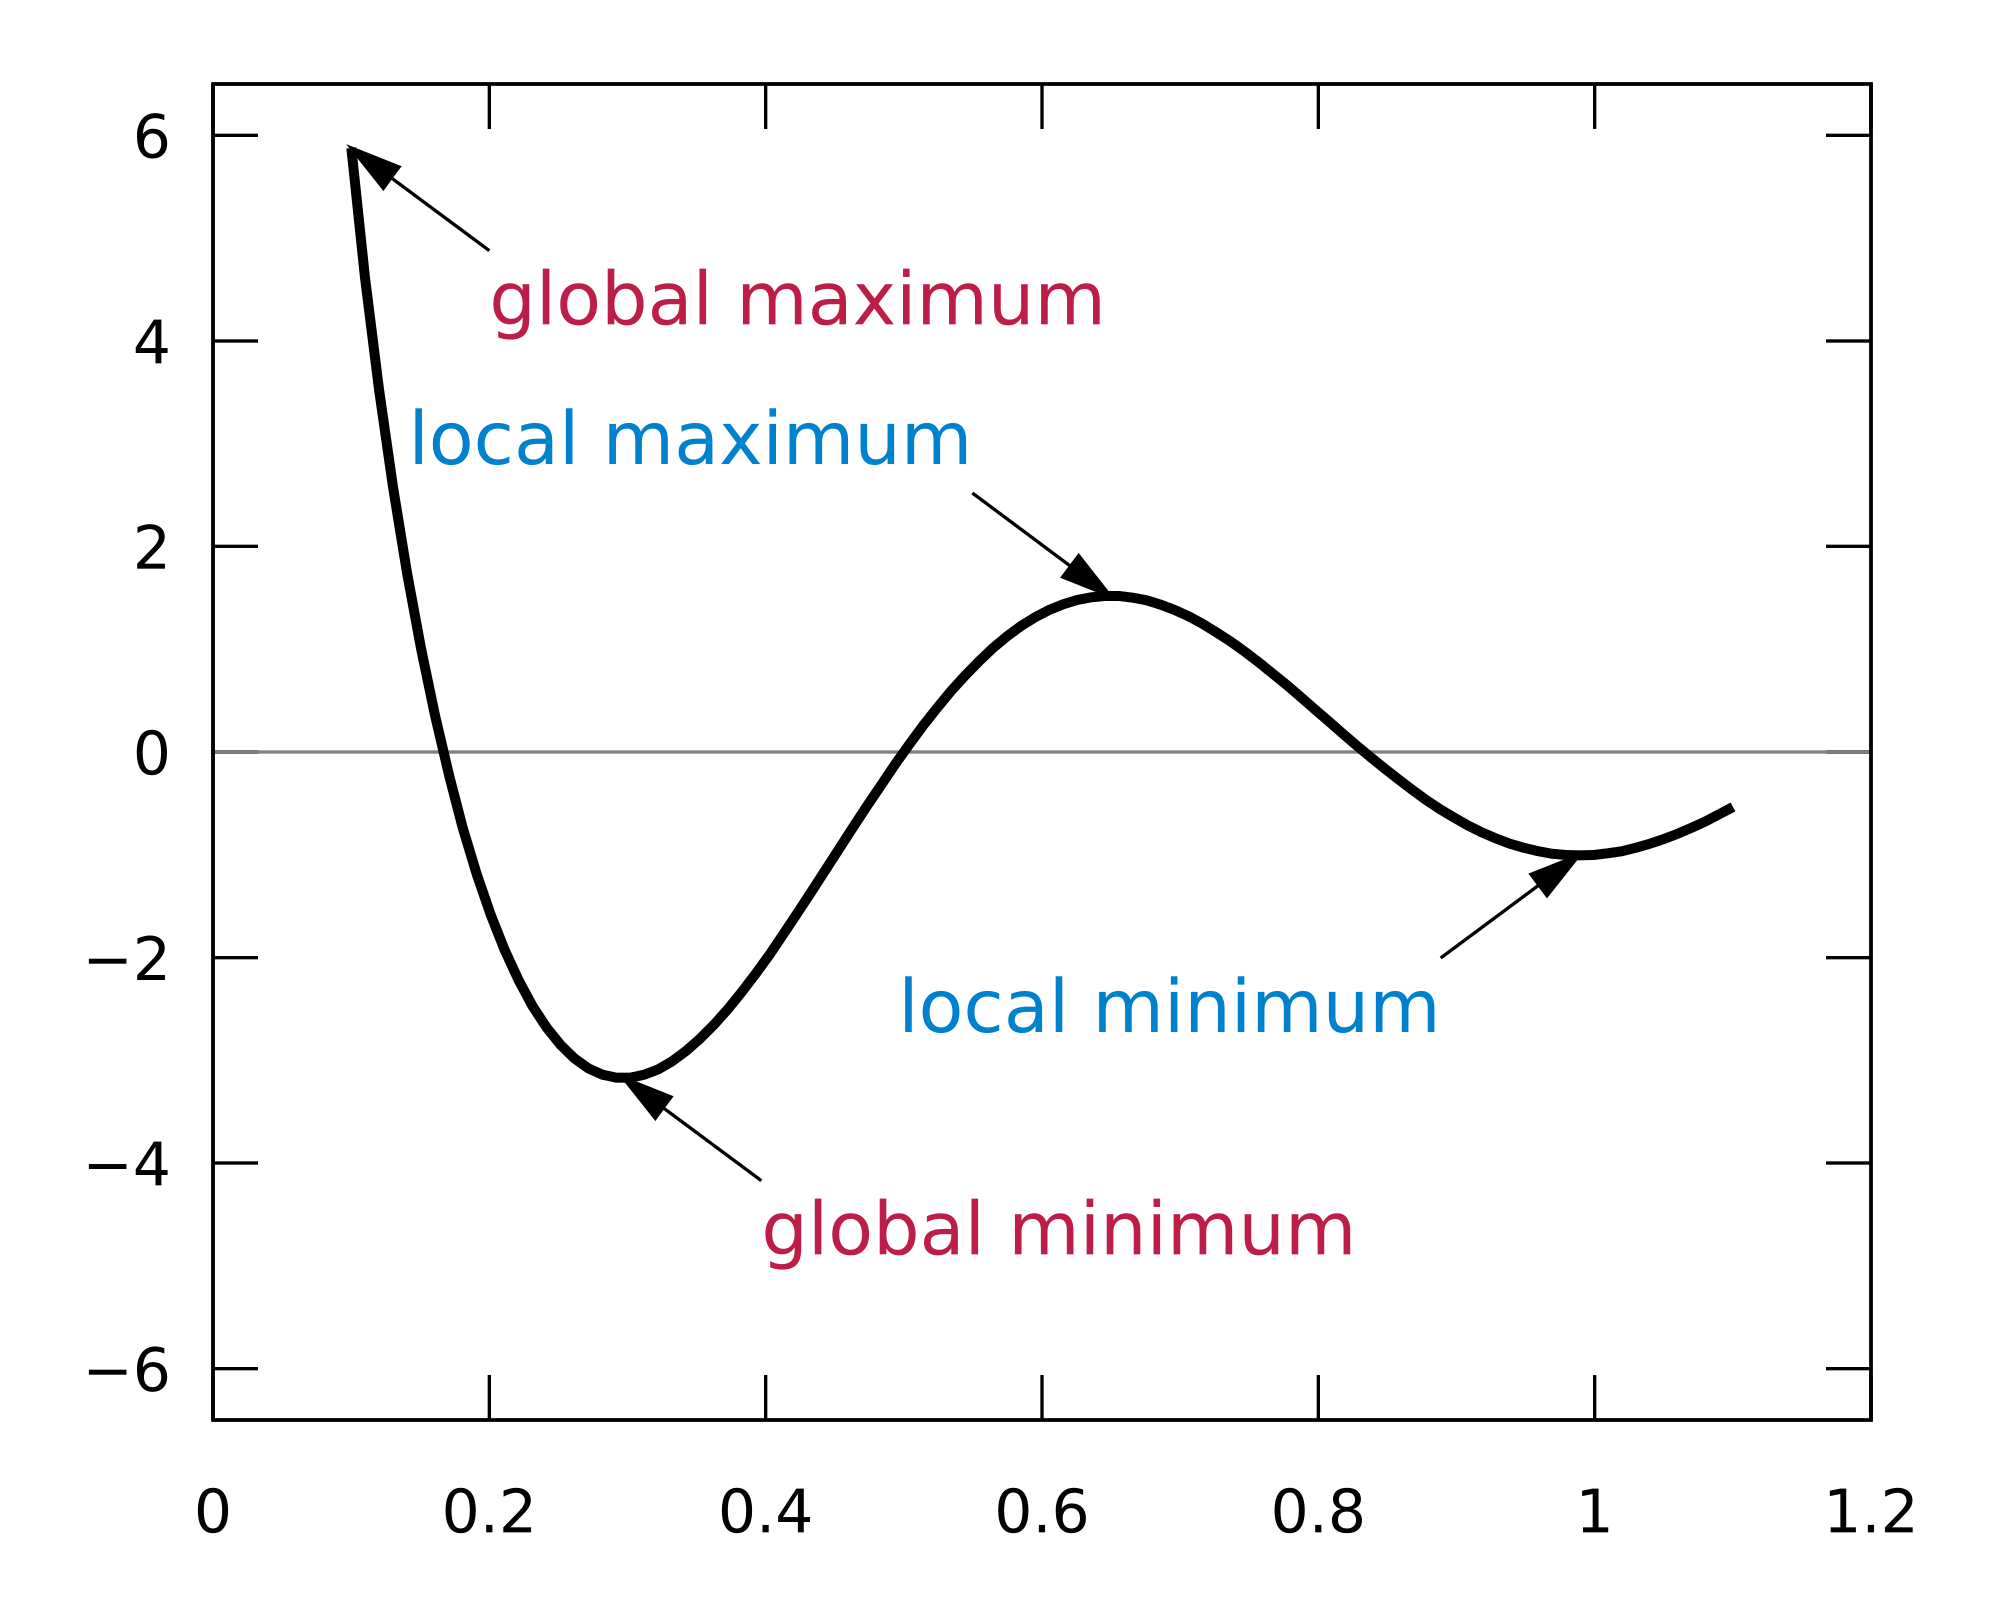
\includegraphics[scale=0.095]{./pictures/local_minima.png}
  \end{center}
\end{frame}

\begin{frame}[c]{Momentum}
  \begin{itemize}
    \item An extension to the backpropagation algorithm
    \item Simply take into account the previous weight update
  \end{itemize}
\end{frame}

\begin{frame}{Simulated annealing}
\begin{itemize}
  \item Start with a large learning rate
  \item Make the learning rate smaller at each iteration
  \item This allows the model to search through a large weight-space before
  converging more precisely.
\end{itemize}
\end{frame}

\begin{frame}{Average multiple networks}
\begin{center}
  \Large{$h_w(x) = \frac{h_{w_1}(x) + \cdots + h_{w_n}(x)}{n}$}
\end{center}
\end{frame}

% momentum
% regularization
